% VerA.web (public) Teχ-Experimente
%
% Copyright © 2015
%	Thorsten Glaser <t.glaser@tarent.de>
%
% Provided that these terms and disclaimer and all copyright notices
% are retained or reproduced in an accompanying document, permission
% is granted to deal in this work without restriction, including un‐
% limited rights to use, publicly perform, distribute, sell, modify,
% merge, give away, or sublicence.
%
% This work is provided “AS IS” and WITHOUT WARRANTY of any kind, to
% the utmost extent permitted by applicable law, neither express nor
% implied; without malicious intent or gross negligence. In no event
% may a licensor, author or contributor be held liable for indirect,
% direct, other damage, loss, or other issues arising in any way out
% of dealing in the work, even if advised of the possibility of such
% damage or existence of a defect, except proven that it results out
% of said person’s immediate fault when using the work as intended.

\documentclass{tarentanleitung}
\usepackage{tikz}
\usetikzlibrary{arrows,backgrounds,fit,positioning,shapes,shadows}
\begin{document}

% VerA.web (public) Installationsanleitung
%
% Copyright © 2015, 2016
%	Thorsten Glaser <t.glaser@tarent.de>
%
% Provided that these terms and disclaimer and all copyright notices
% are retained or reproduced in an accompanying document, permission
% is granted to deal in this work without restriction, including un‐
% limited rights to use, publicly perform, distribute, sell, modify,
% merge, give away, or sublicence.
%
% This work is provided “AS IS” and WITHOUT WARRANTY of any kind, to
% the utmost extent permitted by applicable law, neither express nor
% implied; without malicious intent or gross negligence. In no event
% may a licensor, author or contributor be held liable for indirect,
% direct, other damage, loss, or other issues arising in any way out
% of dealing in the work, even if advised of the possibility of such
% damage or existence of a defect, except proven that it results out
% of said person’s immediate fault when using the work as intended.

% VerA.web Fassung der Installationsanleitung
\newcommand{\vwiaversfassungnr}{4.2}
\newcommand{\vwiaversfassungmonat}{April}
\newcommand{\vwiaversfassungjahr}{2016}

% VerA.web Version
\newcommand{\vwiaverssw}{1.8.43}

% OSIAM Version (Auth-/Resource-Server, nicht Distribution)
\newcommand{\vwiaversosiam}{2.3}
% zugehörige Distribution
\newcommand{\vwiaversodist}{2.4}

% Upgrade von /etc/veraweb (1.4.3.5 oder 1.5.1.4+)
\newif\ifvwconfigsinetcalready
\vwconfigsinetcalreadyfalse

% Installationsanleitung oder nur Upgrade?
\newif\ifupgradeanleitung
\upgradeanleitungtrue

% Textweiche mit/ohne OA
\newif\ifoa
\oafalse

\tarentanleitung
 {Experimente}
 {\vwiaverssw}{\vwiaversfassungnr}{\vwiaversfassungmonat}{\vwiaversfassungjahr}{veraweblogo}

% LaTeX Table of Contents for tarent
%
% Copyright © 2015
%	Thorsten Glaser <t.glaser@tarent.de>
%
% Provided that these terms and disclaimer and all copyright notices
% are retained or reproduced in an accompanying document, permission
% is granted to deal in this work without restriction, including un‐
% limited rights to use, publicly perform, distribute, sell, modify,
% merge, give away, or sublicence.
%
% This work is provided “AS IS” and WITHOUT WARRANTY of any kind, to
% the utmost extent permitted by applicable law, neither express nor
% implied; without malicious intent or gross negligence. In no event
% may a licensor, author or contributor be held liable for indirect,
% direct, other damage, loss, or other issues arising in any way out
% of dealing in the work, even if advised of the possibility of such
% damage or existence of a defect, except proven that it results out
% of said person’s immediate fault when using the work as intended.
%-
% include with 「% LaTeX Table of Contents for tarent
%
% Copyright © 2015
%	Thorsten Glaser <t.glaser@tarent.de>
%
% Provided that these terms and disclaimer and all copyright notices
% are retained or reproduced in an accompanying document, permission
% is granted to deal in this work without restriction, including un‐
% limited rights to use, publicly perform, distribute, sell, modify,
% merge, give away, or sublicence.
%
% This work is provided “AS IS” and WITHOUT WARRANTY of any kind, to
% the utmost extent permitted by applicable law, neither express nor
% implied; without malicious intent or gross negligence. In no event
% may a licensor, author or contributor be held liable for indirect,
% direct, other damage, loss, or other issues arising in any way out
% of dealing in the work, even if advised of the possibility of such
% damage or existence of a defect, except proven that it results out
% of said person’s immediate fault when using the work as intended.
%-
% include with 「% LaTeX Table of Contents for tarent
%
% Copyright © 2015
%	Thorsten Glaser <t.glaser@tarent.de>
%
% Provided that these terms and disclaimer and all copyright notices
% are retained or reproduced in an accompanying document, permission
% is granted to deal in this work without restriction, including un‐
% limited rights to use, publicly perform, distribute, sell, modify,
% merge, give away, or sublicence.
%
% This work is provided “AS IS” and WITHOUT WARRANTY of any kind, to
% the utmost extent permitted by applicable law, neither express nor
% implied; without malicious intent or gross negligence. In no event
% may a licensor, author or contributor be held liable for indirect,
% direct, other damage, loss, or other issues arising in any way out
% of dealing in the work, even if advised of the possibility of such
% damage or existence of a defect, except proven that it results out
% of said person’s immediate fault when using the work as intended.
%-
% include with 「\input{toc.tex}」 after \tarentanleitung{…}…

\addtocontents{toc}{\protect\thispagestyle{fancy}}
\addtolength{\cftsubsecnumwidth}{0.5em}
\addtolength{\cftsubsubsecindent}{0.5em}
\renewcommand{\cftsecleader}{\cftdotfill{\cftdotsep}}
\hypersetup{linkcolor = black}
\tableofcontents
\hypersetup{linkcolor = blue}
\newpage
」 after \tarentanleitung{…}…

\addtocontents{toc}{\protect\thispagestyle{fancy}}
\addtolength{\cftsubsecnumwidth}{0.5em}
\addtolength{\cftsubsubsecindent}{0.5em}
\renewcommand{\cftsecleader}{\cftdotfill{\cftdotsep}}
\hypersetup{linkcolor = black}
\tableofcontents
\hypersetup{linkcolor = blue}
\newpage
」 after \tarentanleitung{…}…

\addtocontents{toc}{\protect\thispagestyle{fancy}}
\addtolength{\cftsubsecnumwidth}{0.5em}
\addtolength{\cftsubsubsecindent}{0.5em}
\renewcommand{\cftsecleader}{\cftdotfill{\cftdotsep}}
\hypersetup{linkcolor = black}
\tableofcontents
\hypersetup{linkcolor = blue}
\newpage


\section{Experimente}

\subsection{tikz/pgf}

\begin{minipage}{\textwidth}

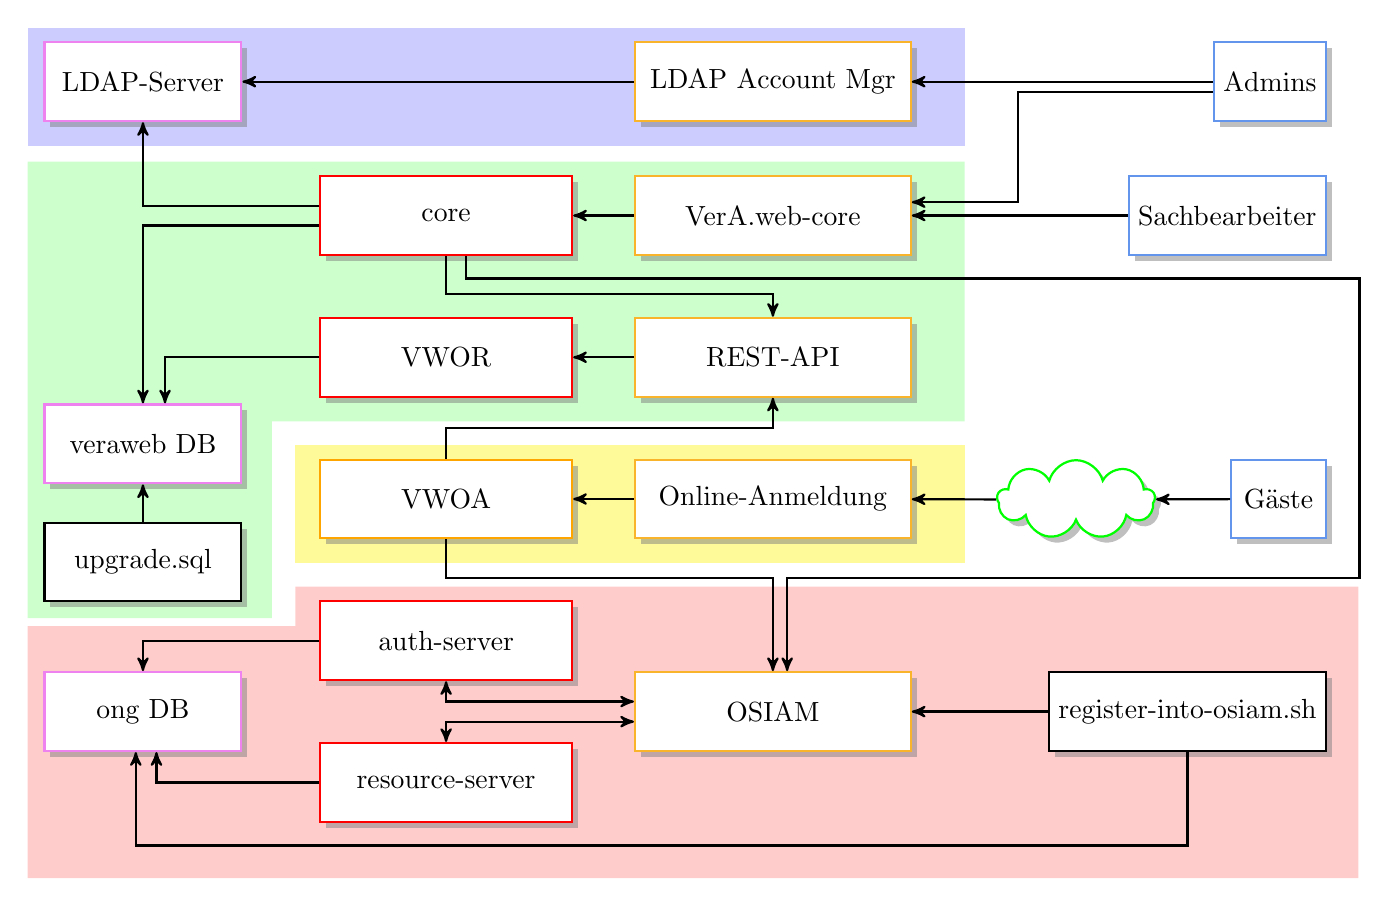
\begin{tikzpicture}[
  >=stealth',
  every node/.style={thick,text=black,fill=white,drop shadow},
  every rectangle node/.style={minimum height=10mm},
  apache/.style={above right,rectangle,draw=Dandelion,minimum width=35mm},
  microsvc/.style={above right,rectangle,draw=Orange,minimum width=32mm},
  webapp/.style={above right,rectangle,draw=red,minimum width=32mm},
  syssvc/.style={above right,rectangle,draw=Violet,minimum width=25mm},
  scrptr/.style={above right,rectangle,draw=black,minimum width=25mm},
  scrptl/.style={above left,rectangle,draw=black,minimum width=25mm},
  people/.style={above left,rectangle,draw=CornflowerBlue,minimum width=12mm},
  acloud/.style={cloud,cloud puffs=9,draw=green,above right,minimum width=20mm,minimum height=10mm},
 ]

% \draw (0mm,0mm) -- (0mm,120mm) -- (175mm,120mm) -- (175mm,0mm) -- (0mm,0mm);

  \fill[red!20] (3mm,3mm) -- (172mm,3mm) -- (172mm,40mm) -- (37mm,40mm) -- (37mm,35mm) -- (3mm,35mm);
  \fill[yellow!40] (37mm,43mm) -- (122mm,43mm) -- (122mm,58mm) -- (37mm,58mm);
  \fill[green!20] (3mm,36mm) -- (34mm,36mm) -- (34mm,61mm) -- (122mm,61mm) -- (122mm,94mm) -- (3mm,94mm);
  \fill[blue!20] (3mm,96mm) -- (122mm,96mm) -- (122mm,111mm) -- (3mm,111mm);

  \node[apache]   (alam)   at ( 80mm,99mm) {LDAP Account Mgr};
  \node[apache]   (acore)  at ( 80mm,82mm) {VerA.web-core};
  \node[apache]   (avwor)  at ( 80mm,64mm) {REST-API};
  \node[apache]   (avwoa)  at ( 80mm,46mm) {Online-Anmeldung};
  \node[apache]   (aosiam) at ( 80mm,19mm) {OSIAM};
  \node[microsvc] (svwoa)  at ( 40mm,46mm) {VWOA};
  \node[webapp]   (score)  at ( 40mm,82mm) {core};
  \node[webapp]   (svwor)  at ( 40mm,64mm) {VWOR};
  \node[webapp]   (sauth)  at ( 40mm,28mm) {auth-server};
  \node[webapp]   (srsrc)  at ( 40mm,10mm) {resource-server};
  \node[syssvc]   (ldap)   at (  5mm,99mm) {LDAP-Server};
  \node[syssvc]   (dbvw)   at (  5mm,53mm) {veraweb DB};
  \node[syssvc]   (dbong)  at (  5mm,19mm) {ong DB};
  \node[scrptr]   (usql)   at (  5mm,38mm) {upgrade.sql};
  \node[scrptl]   (riosh)  at (168mm,19mm) {register-into-osiam.sh};
  \node[people]   (admins) at (168mm,99mm) {Admins};
  \node[people]   (sb)     at (168mm,82mm) {Sachbearbeiter};
  \node[people]   (guests) at (168mm,46mm) {Gäste};
  \node[acloud]   (inet)   at (130mm,48mm) {};

  \draw[thick,->] (admins) -- ([yshift=3mm]alam);
  \draw[thick,->] (alam) -- (ldap);
  \draw[thick,->] ([yshift=-6mm]admins) -| +(-32mm,0mm) |- ([yshift=3mm]acore);
  \draw[thick,->] (acore) -- (score);
  \draw[thick,->] ([yshift=3mm]score) -| (ldap);
  \draw[thick,->] (sb) -- (acore);
  \draw[thick,->] ([yshift=-3mm]score) -| (dbvw);
  \draw[thick,->] ([xshift=4mm]score) |- ++(112mm,-8mm) |- ++(-20mm,-38mm) -| ([xshift=6mm]aosiam);
  \draw[thick,->] (score) |- +(25mm,-10mm) -| (avwor);
  \draw[thick,->] (guests) -- (inet);
  \draw[thick,->] (inet) -- (avwoa);
  \draw[thick,->] (avwoa) -- (svwoa);
  \draw[thick,->] (svwoa) |- +(25mm,9mm) -| (avwor);
  \draw[thick,->] (avwor) -- (svwor);
  \draw[thick,->] (svwor) -| ([xshift=6mm]dbvw);
  \draw[thick,->] (usql) -- (dbvw);
  \draw[thick,<->] ([yshift=3mm]aosiam) -| (sauth);
  \draw[thick,<->] ([yshift=-3mm]aosiam) -| (srsrc);
  \draw[thick,->] (sauth) -| (dbong);
  \draw[thick,->] (srsrc) -| ([xshift=3mm]dbong);
  \draw[thick,->] (riosh) -- +(0mm,-17mm) -| ([xshift=-3mm]dbong);
  \draw[thick,->] (riosh) -- (aosiam);
  \draw[thick,->] (svwoa) |- +(20mm,-10mm) -| (aosiam);

\end{tikzpicture}

\vspace{0.3cm}

\begin{tabu} to \linewidth {rllll}
\rowfont\bfseries\multicolumn{5}{c}{Legende}\\[0.2cm]
 Erste Spalte: & \multicolumn{2}{l}{%
			\tikz \node[thick,rectangle,draw=Violet] {};
			PostgreSQL-Datenbank} &
		 \multicolumn{2}{l}{%
			\tikz \node[thick,rectangle,draw=black] {};
			Skript (Installation/Upgrade)}\\
Zweite Spalte: & \multicolumn{2}{l}{%
			\tikz \node[thick,rectangle,draw=red] {};
			Webservice (WAR) in Tomcat} &
		 \multicolumn{2}{l}{%
			\tikz \node[thick,rectangle,draw=Orange] {};
			Microservice (JAR)}\\
Dritte Spalte: & \multicolumn{4}{l}{%
			\tikz \node[thick,rectangle,draw=Dandelion] {};
			 Apache Webserver (SSL, mod\_jk oder mod\_proxy\_http)}\\
Vierte Spalte: & \multicolumn{2}{l}{%
			\tikz \node[thick,rectangle,draw=CornflowerBlue] {};
			 Nutzergruppe (per Webbrowser)} &
		 \multicolumn{2}{l}{%
			\tikz \node[thick,rectangle,draw=black] {};
			Skript (Installation/Upgrade)}\\
 Schattierung: & \tikz \node[rectangle,fill=red!30] {}; OSIAM &
		 \tikz \node[rectangle,fill=yellow!60] {}; Online-Anmeldung &
		 \tikz \node[rectangle,fill=green!30] {}; VerA.web core &
		 \tikz \node[rectangle,fill=blue!30] {}; LDAP\\
\multicolumn{5}{l}{\footnotesize Zugang für Gäste durch das Internet (Wolke);
		   Administratoren und Sachbearbeiter via Intranet/DMZ/VPN}\\
\end{tabu}

\end{minipage}

\subsection{Seitenbreite}

Wie breit ist die Seite? % 497.92325pt ~= 175 mm (5 Nullen nach dem Komma)
% ein Teχ-Punkt (pt) ist exakt 2540/7227 mm = 0.3̅5̅1̅4̅5̅9̅8̅0̅ mm
% ein Teχ-Punkt (pt) ist exakt 800/803 PostScript-Punkt (pt, Teχ bp) = 0.9̅9̅6̅2̅6̅4̅0̅0̅ bp
% Teχ rechnet intern nur auf ca. 6 Stellen genau, fixed-point, daher vmtl. exakt

\the\textwidth

\subsection{bedingte Ausführung}

Kann ich Text ifdef'en?

\newif\ifosiam
\osiamtrue

\ifosiam
 OSIAM ja2 (ok)
\else
 OSIAM nein2
\fi

\ifosiam
 OSIAM ja1 (ok)
\fi

% \if!osiam ist immer false, \ifnotosiam schmeißt nen Fehler ☹
\ifosiam\else
 OSIAM nein1
\fi

\osiamfalse

\ifosiam
 OSIAM ja2
\else
 OSIAM nein2 (ok)
\fi

\ifosiam
 OSIAM ja1
\fi

% \if!osiam ist immer false, \ifnotosiam schmeißt nen Fehler ☹
\ifosiam\else
 OSIAM nein1 (ok)
\fi

\subsection{Abbildungen}

Gehen Abbildungen? Und wenn ja, wie macht man sie schön?

\begin{figure}[h!]
 \centering
\includegraphics[width=.8\textwidth]{veraweblogo}
% \\\the\textwidth % ändert sich nicht (getestet)
 \caption{Das Veraweb-Logo auf 80\% Breite}
 \label{fig:logovw}
\end{figure}

Hier könnte man noch etwas längeren Text einfügen, zum Beispiel
welchen, der erklärt, warum man hier eine Tilde \~{} statt eines
Leerzeichens verwendet, aber paßt schon so.

\newpage

Allerdings will ich den Umbruch und die Verweise testen, daher
brauche ich hier einen Seitenumbruch.

\begin{figure}[h!]
 \centering
\includegraphics[width=\textwidth]{tarentlogo}
% \\\the\textwidth
 \caption{Das tarent-Logo auf 100\% Breite}
 \label{fig:logotarent}
\end{figure}

In Abbildung~\ref{fig:logovw} sehen Sie das VerA.web-Logo;
Abbildung~\ref{fig:logotarent} verweist auf das neue tarent-Logo.

\subsection{Listing Copy \& Paste}

\begin{minipage}{\textwidth}
Fixed:

\begin{lstdump}[language=sh,columns=fixed]{with fixed}
sudo mkdir -p /etc/veraweb/l10n
sudo install -c -o 0 -g 0 -m 644 l10n/* /etc/veraweb/l10n/
sudo install -c -o 0 -g 0 -m 644 config_ldap_access.xml /etc/veraweb/
sudo -u postgres createdb -E UTF-8 -O veraweb -T template0 veraweb

+---------------------------------------------------+
|                                                   |
| meh                                               |
| meow                                              |
| meh x                                             |
| ieh x                                             |
| iiiiiiiiiiiiiiiiiiiiiiiiiiiiiiiiiiiiiiiiiiiiiiiii |
| i     i     i     i     i       i       i       i |
| i i i i i i i i i i i i i i i i i i i i i i i i i |
| x x x x x x x x x x x x x x x x x x x x x x x x x |
| m m m m m m m m m m m m m m m m m m m m m m m m m |
| mmmmmmmmmmmmmmmmmmmmmmmmmmmmmmmmmmmmmmmmmmmmmmmmm |
| xxxxxxxxxxxxxxxxxxxxxxxxxxxxxxxxxxxxxxxxxxxxxxxxx |
| a!b"c#d$e%f&g'h(i)j*k+l-m/n^o_p`q~r\s[t{u|v?w^x<y |
| a b c d e f g h i j k l m n o p q r s t u v w x y |
+---------------------------------------------------+

\end{lstdump}
\end{minipage}

\begin{minipage}{\textwidth}
Flexible:

\begin{lstdump}[language=sh,columns=flexible]{with flexible}
sudo mkdir -p /etc/veraweb/l10n
sudo install -c -o 0 -g 0 -m 644 l10n/* /etc/veraweb/l10n/
sudo install -c -o 0 -g 0 -m 644 config_ldap_access.xml /etc/veraweb/
sudo -u postgres createdb -E UTF-8 -O veraweb -T template0 veraweb

+---------------------------------------------------+
|                                                   |
| meh                                               |
| meow                                              |
| meh x                                             |
| ieh x                                             |
| iiiiiiiiiiiiiiiiiiiiiiiiiiiiiiiiiiiiiiiiiiiiiiiii |
| i     i     i     i     i       i       i       i |
| i i i i i i i i i i i i i i i i i i i i i i i i i |
| x x x x x x x x x x x x x x x x x x x x x x x x x |
| m m m m m m m m m m m m m m m m m m m m m m m m m |
| mmmmmmmmmmmmmmmmmmmmmmmmmmmmmmmmmmmmmmmmmmmmmmmmm |
| xxxxxxxxxxxxxxxxxxxxxxxxxxxxxxxxxxxxxxxxxxxxxxxxx |
| a!b"c#d$e%f&g'h(i)j*k+l-m/n^o_p`q~r\s[t{u|v?w^x<y |
| a b c d e f g h i j k l m n o p q r s t u v w x y |
+---------------------------------------------------+

\end{lstdump}
\end{minipage}

\begin{minipage}{\textwidth}
Full Flexible:

\begin{lstdump}[language=sh,columns=fullflexible]{with fullflexible}
sudo mkdir -p /etc/veraweb/l10n
sudo install -c -o 0 -g 0 -m 644 l10n/* /etc/veraweb/l10n/
sudo install -c -o 0 -g 0 -m 644 config_ldap_access.xml /etc/veraweb/
sudo -u postgres createdb -E UTF-8 -O veraweb -T template0 veraweb

+---------------------------------------------------+
|                                                   |
| meh                                               |
| meow                                              |
| meh x                                             |
| ieh x                                             |
| iiiiiiiiiiiiiiiiiiiiiiiiiiiiiiiiiiiiiiiiiiiiiiiii |
| i     i     i     i     i       i       i       i |
| i i i i i i i i i i i i i i i i i i i i i i i i i |
| x x x x x x x x x x x x x x x x x x x x x x x x x |
| m m m m m m m m m m m m m m m m m m m m m m m m m |
| mmmmmmmmmmmmmmmmmmmmmmmmmmmmmmmmmmmmmmmmmmmmmmmmm |
| xxxxxxxxxxxxxxxxxxxxxxxxxxxxxxxxxxxxxxxxxxxxxxxxx |
| a!b"c#d$e%f&g'h(i)j*k+l-m/n^o_p`q~r\s[t{u|v?w^x<y |
| a b c d e f g h i j k l m n o p q r s t u v w x y |
+---------------------------------------------------+

\end{lstdump}
\end{minipage}

\section{Nicht-ASCII-Zeichen in Listings}

\begin{minipage}{\textwidth}
Ein minimaler – deutsche Umlaute, sonstige häufige Zeichen – Test:

\begin{lstdump}[language=sh]{non-ASCII chars}
# © 2015 “mirabilos”™ -- tarent §1 20°
echo 'Ah nah, "dummlicher" FuB. Uberdem droge Arbeit. Teste: |'
echo 'Äh näh, „dümmlicher“ Fuß. Überdem dröge Arbeit. Teste: |'
echo 'oO0 Il1 – ‘`’ ist doof. Öh… mach’ halt mal. Alignment: |'
echo "oO0 Il1 - '`' ist doof. Oh. mach' halt mal. Alignment: |"
\end{lstdump}
\end{minipage}

\end{document}
